\documentclass[10pt]{article}
\usepackage[margin=1in]{geometry}

%% Language and font encodings
\usepackage[utf8]{inputenc}
\usepackage[T1]{fontenc}

% graphics and colors
\usepackage{graphicx}
\usepackage{xcolor}

\usepackage{enumerate}
\usepackage{verbatim}

%% Math!
\usepackage{amsmath,amssymb,amsfonts,amsthm}
\usepackage{mathtools}
\usepackage{tikz}
\usetikzlibrary{trees}
\usepackage[linesnumbered,ruled]{algorithm2e}
\DeclarePairedDelimiter\ceil{\lceil}{\rceil}
\DeclarePairedDelimiter\floor{\lfloor}{\rfloor}

% some basic definitions
\newcommand{\pct}{\mathbin{\%}}
% makes ":=" aligned better
\usepackage{mathtools}
\mathtoolsset{centercolon}
\newcommand{\concat}{\|}
\DeclareMathOperator*{\argmin}{argmin}
\DeclareMathOperator*{\avg}{avg}
\DeclareMathOperator*{\all}{all}
\renewcommand{\O}{\mathcal{O}}

\usepackage{varwidth}

\title{CS 478 Lab Reports}
\author{
Ekstedt, Andrew\\
\texttt{ekstedta@oregonstate.edu}
}
\date{\today}
\begin{document}
\maketitle

\section{Lab 1: Puzzles}
\subsection{Introduction}

We implemented a simple client-server puzzle scheme to mitigate denial of service attacks, based on brute-forcing $n$ bits of a hash \cite{juels}.

\subsection{Benchmarks}

We measured how long it took the client to solve puzzles as the number $n$ of puzzle bits increased. For each $n$ we made 20 requests to the server and timed how long they took. Up to 7 bits there is approximately no visible effect, but after 7 the time to solve each puzzle goes up by about a factor of two for each bit, which is what we expect. See Table~\ref{tab:puzzles}. 

\begin{table}[h]
\centering
\begin{tabular}{cccc}
\hline
Bits & Average solve time & Requests per second \\
\hline
4 & 0.5ms & 1845\\
5 & 0.55ms & 1753\\
6 & 0.70ms & 1346\\
7 & 0.70ms & 1348	\\
8 & 1.0ms & 992\\
9 & 1.7ms& 557 \\
10 & 2.1ms & 470 \\
11 & 4.3ms & 227.8\\
12 & 8.2ms & 121.5\\
13 & 14.2ms & 70.1 \\
14 & 29.2ms & 34.2 \\
15 & 65.1ms & 15.3 \\
16 & 86.7ms & 11.5 \\
17 & 207ms & 4.8 \\
\hline
\end{tabular}
\caption{Benchmark results for client-server puzzles.}
\label{tab:puzzles}
\end{table}

\clearpage
\section{Lab 2: HORS}
\subsection{Introduction}

We implemented PQ, a stateful many-time hashed-based signature scheme based on HORS.
See algorithm~\ref{alg:pq} for the complete algorithm.

The main limitation of HORS is that each key pair can only be used once;
we extend HORS and turn it into a $d$-time signature scheme.
The main idea behind PQ is to generate $d$ HORS keys, but instead of transmitting all $d\times t$ elements of the signature, we compute a Merkle tree over the leaves and use the root as the public key.

PQ contains three main improvements over HORS:
\begin{enumerate}
\item We use a Merkle tree to verify signatures, allowing us to shrink the size of the public key.
\item We use a PRF to generate the leaves of the Merkle tree, allowing us to shrink the size of the private key.
\item The Merkle tree is generated over $d\cdot t$ leaves instead of just $t$ leaves, allowing us to sign $d$ messages.
\end{enumerate}

We present a diagram of a Merkle tree on top of a single HORS key in Figure~\ref{fig:hors}. The root of the tree is capable of verifying all the leaves, allowing us to distribute just the root as the public key. The secret elements $s_i$ are generated from a seed value as $s_i = F_z(i)$. Figure~\ref{fig:pq} shows the tree in PQ. This can be view as a series of $d$ independent, virtual HORS signature trees, connected together with another Merkle tree on top, or it can be viewed as a single Merkle tree of $d\times t$ elements.

\begin{algorithm}
\caption{The PQ signature scheme}
\label{alg:pq}
\SetKwProg{Fn}{func}{}{end}
Let $F : \{0,1\}^\lambda \times \{0,1\}^* \to \{0,1\}^{k\log_2 t}$ be a secure PRF.\\
Let $H : \{0,1\}^* \to \{0,1\}^\lambda$ be a secure hash function.\\
Let $t$ be the number of HORS key elements.\\
Let $k$ be the number of HORS signature elements.\\
Let $d$ be the maximum number of messages.\\
\Fn{PQ.Keygen}{
	$z \gets \{0,1\}^\lambda$ \\
    $st \gets 1$ \\
    \For{$i$ from $1$ to $d\times t$} {
    	$s_i \gets F_z(i)$\\
        $v_i \gets H(s_i)$
    }
    $R \gets Merkle.Create(v_1, \ldots, v_{d\times t})$ \\
    \Return { $sk = (z,st,d), pk = (R,d)$ }
}
\Fn{PQ.Sign(m,sk)}{
	\If{$st > d$}{
    	abort
    }
    $(h_1\|\ldots\|h_k) \gets H(m)$ \\
    \For{$j \gets 1$ to $k$}{
    	$i_j \gets (st - 1)\times t + h_j$ \\
        $s_{i_j} \gets F_z(i_j)$\\
        $v_{i_j} \gets H(s_{i_j})$\\
        $P_{i_j} \gets Merkle.Path(v_{i_j})$
    }
    $st \gets st + 1$\\
    \Return { $\sigma = (s_{i_1}, P_1, \ldots, s_{i_j}, P_{i_j})$ }
}
\Fn{PQ.Verify(m,$\sigma$,pk)}{
    $(h_1\|\ldots\|h_k) \gets H(m)$ \\
    \For{$j \gets 1$ to $k$}{
        $v_j \gets H(s_{i_j})$\\
        $b_i \gets Merkle.Verify(v_{i_j})$
    }
    $b \gets \all\limits_{i\in 1..j}{b_i} = 1$ \\
    \Return { b }
}
\end{algorithm}



\begin{figure}
\centering
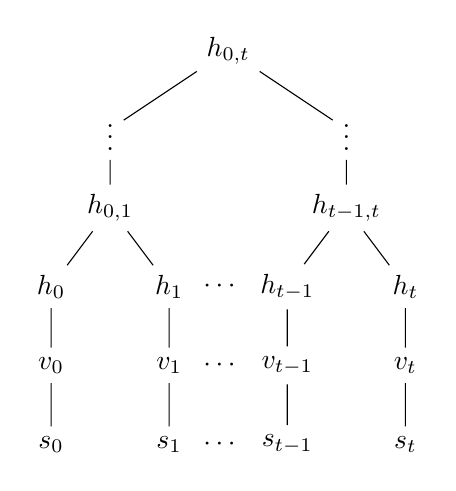
\begin{tikzpicture}[level distance=1cm,
  level 1/.style={sibling distance=3cm},
  level 2/.style={sibling distance=1.5cm}]
  \node {$h_{0,t}$}
  	child {node {$\vdots$}
    child {node {$h_{0,1}$}
      child {node {$h_0$} child { node {$v_0$} child { node { $s_0$ }} }}
      child {node (h1) {$h_1$} child { node (v1) {$v_1$} child { node (s1) { $s_1$ } }}}
    }}
    child {node {$\vdots$}
    child {node {$h_{t-1,t}$}
      child {node (h2) {$h_{t-1}$} child { node (v2) {$v_{t-1}$} child { node (s2) {$s_{t-1}$} } }}
      child {node {$h_t$}     child { node {$v_t$}     child { node {$s_t$} }     }}
    }};
	\path (h1) -- (h2) node [midway] {$\cdots$};
	\path (v1) -- (v2) node [midway] {$\cdots$};
	\path (s1) -- (s2) node [midway] {$\cdots$};
\end{tikzpicture}
\caption{A Merkle tree on top of HORS. The bottom two rows of the tree are the HORS public key and private key elements. The remaining rows are intermediate nodes in the Merkle tree.}
\label{fig:hors}
\end{figure}

\begin{figure}
\centering
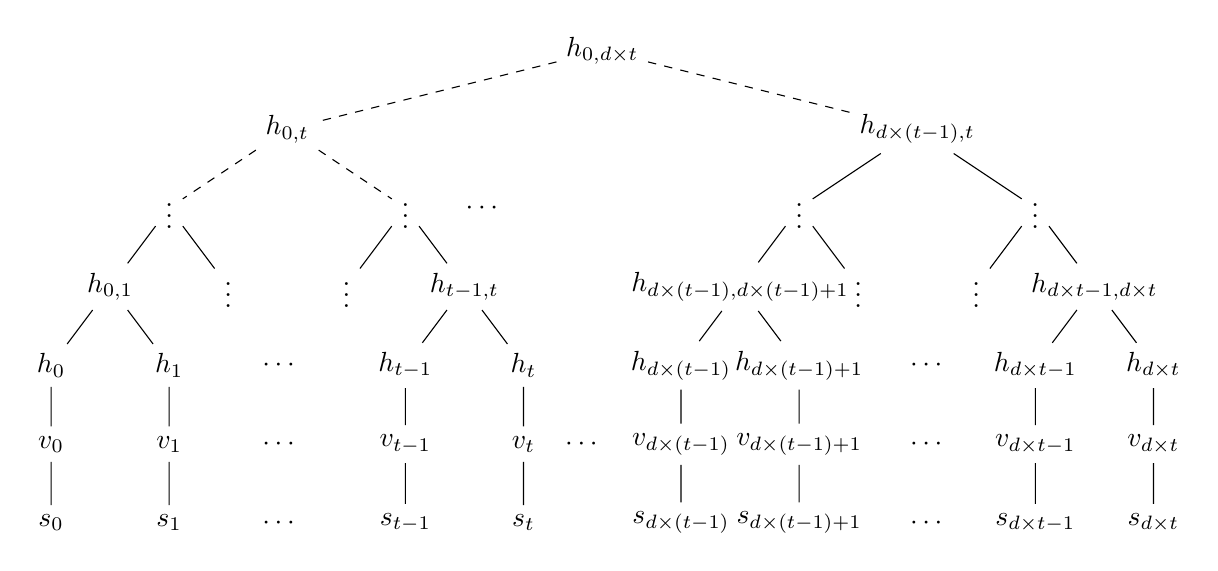
\begin{tikzpicture}[level distance=1cm,
  level 1/.style={sibling distance=8cm},
  level 2/.style={sibling distance=3cm},
  level 3/.style={sibling distance=1.5cm}]
  \node {$h_{0,d\times t}$}
  	child [dashed] {
      node {$h_{0,t}$}
      child {node (dot1) {$\vdots$}
        child [solid] {node {$h_{0,1}$}
          child {node {$h_0$} child { node {$v_0$} child { node { $s_0$ }} }}
          child {node (h1a) {$h_1$} child { node (v1a) {$v_1$} child { node (s1a) { $s_1$ } }}}
        }
      	child [solid] {node {$\vdots$}}
      }
      child {node {$\vdots$}
      	child [solid] {node {$\vdots$}}
        child [solid] {node {$h_{t-1,t}$}
          child {node (h2a) {$h_{t-1}$} child { node (v2a) {$v_{t-1}$} child { node (s2a) {$s_{t-1}$} } }}
          child {node {$h_t$}     child { node (mid1) {$v_t$}     child { node {$s_t$} }     }}
        }}
    }
    child [dashed] {
      node {$h_{d\times(t-1),t}$}
      child [solid] {node (dot2) {$\vdots$}
        child {node {$h_{d\times (t-1),d\times(t-1)+1}$}
          child {node {$h_{d\times(t-1)}$}
              child { node (mid2) {$v_{d\times(t-1)}$}
              child { node {$s_{d\times(t-1)}$}} }}
          child {node (h1b) {$h_{d\times(t-1)+1}$}
              child { node (v1b) {$v_{d\times(t-1)+1}$}
              child { node (s1b) {$s_{d\times(t-1)+1}$} }}}
        }
      	child {node {$\vdots$}}}
      child [solid] { node {$\vdots$}
      	child [solid] {node {$\vdots$}}
        child [solid] {node {$h_{d\times t-1,d\times t}$}
          child {node (h2b) {$h_{d\times t - 1}$}
              child { node (v2b) {$v_{d\times t - 1}$}
              child { node (s2b) {$s_{d\times t - 1}$} }}}
          child {node {$h_{d\times t}$} 
              child { node {$v_{d\times t}$}
              child { node {$s_{d\times t}$} }}}
        }}
     };
 
  \path (mid1) -- (mid2) node [midway] {$\cdots$};
  \path (dot1) -- (dot2) node [midway] {$\cdots$};
  \path (h1a) -- (h2a) node [midway] {$\cdots$};
  \path (v1a) -- (v2a) node [midway] {$\cdots$};
  \path (s1a) -- (s2a) node [midway] {$\cdots$};
  \path (h1b) -- (h2b) node [midway] {$\cdots$};
  \path (v1b) -- (v2b) node [midway] {$\cdots$};
  \path (s1b) -- (s2b) node [midway] {$\cdots$};
\end{tikzpicture}
\caption{A Merkle tree in PQ. We can view this as $d$ independent Merkle trees with $t$ elements, with another Merkle tree on top.}
\label{fig:pq}
\end{figure}

\subsection{Tradeoffs}

PQ trades increased signing and verification time for a smaller key size.

The use of a Merkle tree gives us constant-time public keys at the cost of an additional factor of $\log t$ during verification, and an additional $\log t$ factor for signature size due to the need to transmit the Merkle path for each signature element. The advantage is that public keys are constant-size, compared to $d*k$ for a $d$-time HORS scheme.

The biggest disadvantage is the increased signing time. Signing a message requires traversing the entire Merkle tree for each signature element, at a cost of $k*d*t$ compared to $t$ for basic HORS.

Another disadvantage is the need to keep state on the signer side. This is because we must not reuse a HORS key that we have already used.

A table of the big O numbers for key size, signing time, and verification time are given in Table~\ref{tab:hors}


\subsection{Benchmarks}

\begin{table}
\begin{tabular}{ccccccc}
\hline
	 & Secret key size & Public key size & Signature Size & Keygen time & Signing time & Verify time \\
\hline
HORS & $\O(t)$ & $\O(t)$ & $\O(k)$ & $\O(t)$ & $\O(k)$ & $O(k)$ \\
d-HORS & $\O(dt)$ & $\O(dt)$ & $\O(k)$ & $\O(t)$ & $\O(k)$ & $O(k)$ \\
PQ	 & $\O(1)$ & $\O(1)$ & $\O(k \log t)$ & $\O(dt)$ & $\O(kdt)$ & $O(k \log t)$ \\
\hline
HORS & 8192 bits & 8192 bits & \\
PQ	  
(d=2) & 256 bits & 256 bits & & 10ms & 136ms & 0.77ms \\
(d=4) & $\vdots$ & $\vdots$ & & 21ms & 271ms & 0.84ms \\
(d=8) & & &  & 42ms & 546ms & 0.91ms \\
(d=16) & & & & 83ms & 1052ms & 0.95ms \\
(d=32) & & & & 166ms & 2145ms & 1ms \\
\hline
\end{tabular}
\caption{Comparison of HORS and PQ. $d$-HORS is a trivial variant of HORS which generates $d$ separate keys to sign $d$ messages. Assuming $H$ is a 256-bit hash, t=1024 and k=32. }
\label{tab:hors}
% k = 32; \lambda = 256
\end{table}

We benchmarked our implementation of PQ and compared it to straight HORS signatures. See Table~\ref{tab:hors}

\begin{comment}
flip3% make && ./main -d 2
make: Nothing to be done for `all'.
verified sig 0
verified sig 1
did not verify bad msg with sig 0
keygen took 10ms
signing took 136ms
signing took 133ms
verify took 766µs
flip3% make && ./main -d 4
make: Nothing to be done for `all'.
verified sig 0
verified sig 1
did not verify bad msg with sig 0
keygen took 21ms
signing took 271ms
signing took 270ms
verify took 843µs
flip3% make && ./main -d 8
make: Nothing to be done for `all'.
verified sig 0
verified sig 1
did not verify bad msg with sig 0
keygen took 42ms
signing took 546ms
signing took 545ms
verify took 914µs
flip3% make && ./main -d 16
make: Nothing to be done for `all'.
verified sig 0
verified sig 1
did not verify bad msg with sig 0
keygen took 83ms
signing took 1052ms
signing took 1055ms
verify took 946µs
flip3% make && ./main -d 32
make: Nothing to be done for `all'.
verified sig 0
verified sig 1
did not verify bad msg with sig 0
keygen took 166ms
signing took 2145ms
signing took 2134ms
verify took 1ms
\end{comment}

\clearpage
\section{Lab 3: Digital Forensic Tool}

For lab 3, we implemented a mini digital forensic tool which synthesizes a number of different networking and cryptography techniques that we covered in class.

There are 6 properties that we desire from the tool. We enumerate those properties below, along with a rationale for how the tool satisfies that property.

% Main Idea
%	explain each desired property

\begin{itemize}
\item \textbf{Compromise resiliency}. The sensor should be secure against compromise. This is, if an adversary is able to take over the tool, we do not want stored messages to be revealed. We achieve this by continually refreshing the key stored on the device by hashing it with a secure hash. This way, even if the adversary learns the current key, they cannot recover old keys and so cannot decrypt old messages.
\item \textbf{All-or-nothing verification}
Messages are sent in batches; an adversary should not be able to selectively delete messages from a batch without being detected (nothing can prevent an adversary from blocking all messages). We achieve this property by sending a single authentication tag which covers all the messages in a batch. If even one message is deleted or changed, verification will fail.
\item \textbf{Authentication and integrity}
An adversary should not be able to spoof messages. We achieve this property by including an authentication tag with the messages, as above.
\item \textbf{Compression}
Stored messages should be compressed to save space. We achieve this property by using Huffman coding to compress each message.
\item \textbf{Aggregate authentication}
The authentication tag should use only a constant-size amount of storage on the device, even if there are many stored messages. We achieve this property by computing aggregating the authentication tags for each message in a hash chain. Only the last value in the chain is stored and sent to the collector.
\item \textbf{Packet loss resiliency}
The protocol should be usable on a noisy network; this is, the collector should be able to recover the messages even if a few packets are lost. We achieve this property by using Rabin information dispersal to split the messages into $t$ packets such that the message can be recovered even if only $n$ of $t$ are received.
\end{itemize}

% Why this particular order?
We apply operations in the following order when sending (and the reverse order when receiving).
\begin{enumerate}
\item Compression
\item Encryption
\item Authentication
\item Redundancy
\end{enumerate}

Compression must come before encryption because encrypted data cannot be compressed (it is indistinguishable from random data). Authentication should come after encryption because Encrypt-Then-MAC is the only order that has been proven CCA-secure. Redundancy must be applied after encryption (before decryption) because you cannot decrypt data that is missing or corrupted. 

\subsection{Benchmarks}

  We timed how long it took to send messages with this scheme for a variety of message sizes. Results are summarized in Table~\ref{tab:lab3}

\begin{table}
\centering
\begin{tabular}{lcc}
\hline
Message & Message size & Decryption time \\
\hline
64k bytes of the letter "a" & 64000 B & 3ms \\
64k bytes of the letter "a" (1000 messages) & 64000000 & 3200ms \\
64k bytes of the unix dictionary & 64000 B & 23ms \\
entire unix dictionary & 3571894 B & 1100ms \\
jpeg image & 3475052 B & 1200ms \\
\hline
\end{tabular}
\caption{Benchmark results for lab 3. Rabin parameters: $t=8$, $l=4$}
\label{tab:lab3}
\end{table}


\bibliographystyle{IEEEtran}
\bibliography{main}{}

\end{document}
